%% \chapter[htoc-titlei][hhead-titlei]{htitlei}
%% -----------------------------------------------------------------------------
\chapter[The Large Hadron Collider][The Large Hadron Collider]{The Large Hadron Collider}
%test
Production of a sufficient number of high energy collisions to adequately explore
particle physics at the electro-weak scale required the development of one
of the most complex machines ever built, the Large Hadron Collider or LHC. This chapter
provides a very brief overview of the machine with particular focus on the 2012
dataset of proton-proton collisions it enabled. 
The technology involved in the development of the LHC and very breifly
touched upon in this chapter is an enormous achievement
it its own right and is documented in detail here \cite{1748-0221-3-08-S08001,Pettersson:291782,Linnecar:1176380}. 


\section{The Large Hadron Collider}

The LHC is the world's highest energy particle accellerator 
and is located 100m underneath the Franco-Swiss border at the European Organization
for Nuclear Research (CERN) in a 26.7 km tunnel. 

The LHC is a ciruclar 
machine capable of accelerating beams of protons and colliding them at center of mass 
energies up to $\sqrt{s} = 14 TeV$ at 4 collision sites around the ring, where 4 experiments
are housed (ATLAS\cite{ATLAS_detector}, CMS\cite{748-0221-3-08-S08004}, LHCb\cite{1748-0221-3-08-S08005}, and ALICE\cite{1748-0221-3-08-S08002)}. Figure \ref{figure:lhc_lhc} is a diagram
of the layout of the LHC and its experiments\cite{Team:40525}. The LHC also operates in a modes with beams of 
heavy ions. The LHC is composed of thousands of super-conducting Niobium-Titantium 
magnets, cooled to 2.7$^\circ$ C with liquid Helium, which steer and focus the 
particle beams, and a superconducting resonant-frequency (RF) cavity,which boosts the beam
to higher energies. 

% magnets
\begin{figure}[!t]
\centering 
\includegraphics[width=0.35\textwidth]{figs/lhc.pdf}
\caption{ Diagram of the Large Hadron collider and location of the 4 main experiments (ATLAS, CMS, LHCb, and ALICE). Around
  the ring. The diagram also shows the location of the SPS, the final booster ring the accelerator complex that accelerates
    the protons to 450 GeV before injection into the LHC. 
}
\label{figure:lhc_lhc}
\end{figure}



\subsection{The Accelerator Complex}

The accelerator complex is a progressive series of machines that progressively boost
the particle beams to their final beam energy and intenstiy.
Protons are obtained from hydrogen atoms and are accelerated to 50 MeV using the
Linac2, before being injected into the Proton-Synchrotron Booster (PSB). In
the PSB the protons are accelerated to energies of 1.4 GeV for injection
in to the Proton-Synchrotron (PS). The PS accelerates the protons to 25 GeV
and dumps bunches into the Super Proton Synchrotron (SPS), where they 
are accelerated to 450 GeV and finally dumped into the LHC. 

\subsection{Beam Parameters and Collisions} 

For the physics studied at the ATLAS experiment, the two most important parameters of
the collisions provided by the LHC are the center of mass energy and instantaneous luminosity.
High center of mass energies are necessary for the production
of new high mass particles, and because the consitutents of the actual collisions
are the partons of the proton, the CME of the collisions must in general
be much higher than the mass of the particles needed to be produced. The

\begin{figure}[!t]
\centering 
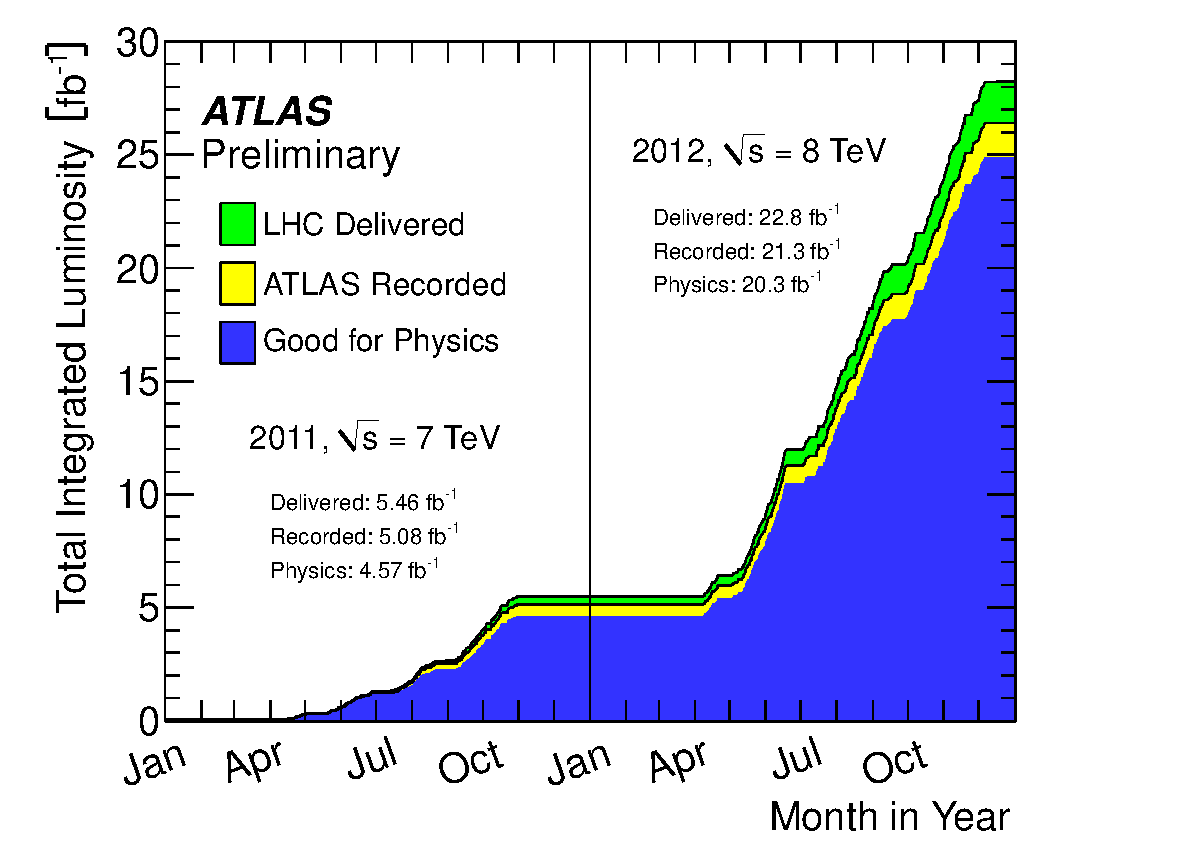
\includegraphics[width=0.35\textwidth]{figs/intlumivstime2011-2012DQ.pdf}
\caption{ Plot showing the accumulation of the integrated lumonisity delivered to the ATLAS experiment over 2011 and 2012. The rough size of the usable, physics ready dataset for 2012 is 20 $fb^-1$ and is the dataset used for the following analysis. 
}
\label{figure:lhc_lumi}
\end{figure}
The instantaneous luminosty of the collisions, \mathscr{L}, is a measure of the
collision rate. The integrated luminosity over time is a measure of the size
of the dataset and when multiplied by the cross-section of a particular process
gives the total number of expected events produced for that process.
Instantaneous luminosity depends on the number of colliding bunches of protons,
the intensity of those bunches, the revolution
frequency, and the nomralized transvserse spread of the beam in momentum and position
phase space, called the emmitance, and the transverse beam size. The LHC has the
option for colliding beams with 2808 bunches of protons, each with around $10^11$ protons,
at a rate of one bunch collision every 25 ns, or 40 MHz. These correspond
to a design luminosity of around $10^34$ cm$^{2}$ s$^-1$ or 10 nb$^-1$ s$^-1$
  
\section{The 2012 Dataset} 

The LHC successfully produced datasets for physics studies in 2010, 2011 and 2012. The 2012 
proton-proton dataset was delivered with collisions with a CME of 8 TeV with bunch collisions
every 50 ns and reached a total integrated luminosity of around ~20 fb$^-1$ \cite{Aad:2013ucp}.
Figure\ref{figure:lhc_lumi} shows the accumulation of this dataset over time. 
The full LHC design energy was never reached due to worries about faulty dipole
connections invovled in the unexpected quenching of the magnets in 2008. Despite doubling
the bunch spacing (thereby halving the bunch collision frequency), the lumonisty neared
the design lumonisty due to unexpected improvements in the transverse beam profile\cite{Carli:1424362}. This increased
the amout of pile-up, or number of collisions per bunch crossing and in general collision
events were busier due to these multiple interactions\cite{}. Figure \ref{figure:lhc_pileup} shows
the average number of interaction per bunch crossing for the 2011 and 2012 datasets. The 2012
dataset shows an average of 20-25 interactions. 

\begin{figure}[!t]
\centering 
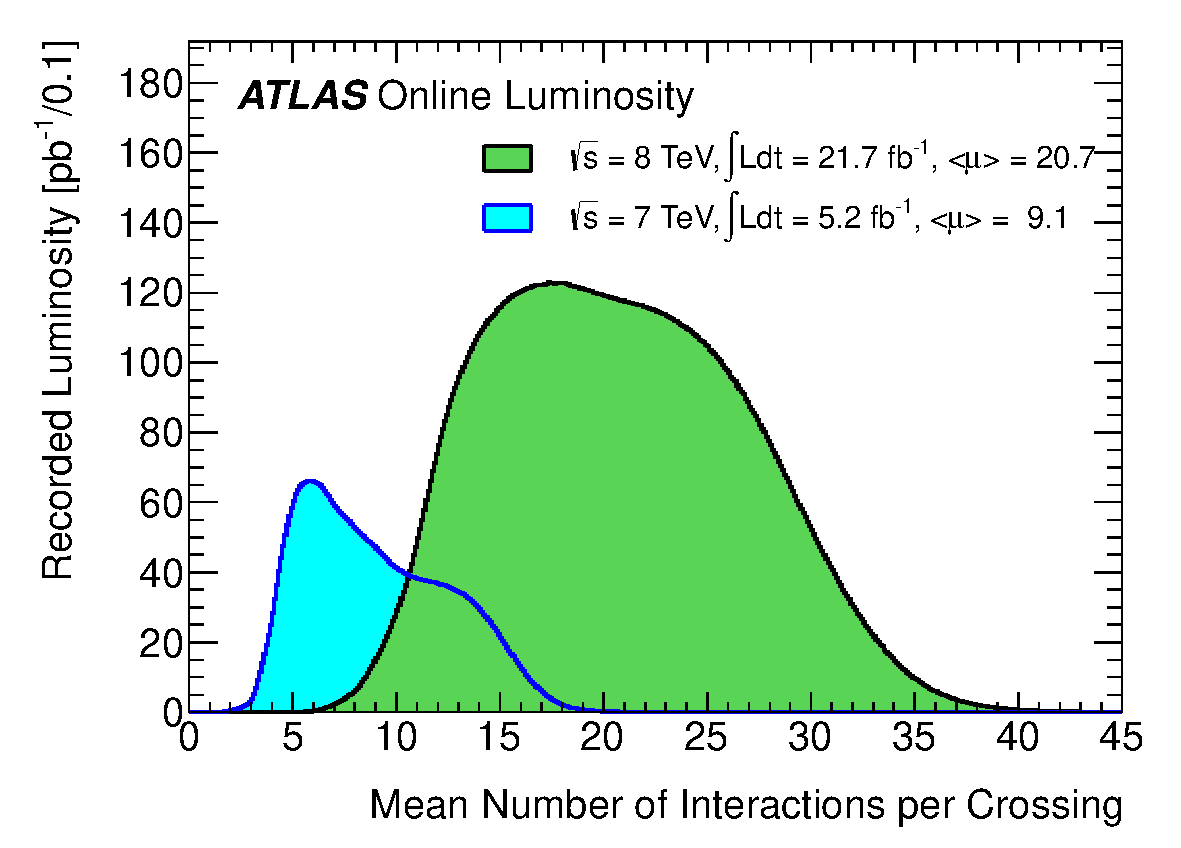
\includegraphics[width=0.35\textwidth]{figs/mu_2011_2012-dec.pdf}
\caption{ The average number of interactions per bunch-crossing for the 2012 and 2011 LHC proton-proton dataset. Most of these interactions are unintersting but leave energetic signatures in particle detectors called pile-up which interfere with measurements}\label{figure:lhc_pileup}

